%%%% ijcai18.tex

\typeout{IJCAI-18 Instructions for Authors}

% These are the instructions for authors for IJCAI-18.
% They are the same as the ones for IJCAI-11 with superficical wording
%   changes only.

\documentclass{article}
\pdfpagewidth=8.5in
\pdfpageheight=11in
% The file ijcai18.sty is the style file for IJCAI-18 (same as ijcai08.sty).
\usepackage{ijcai18}

% Use the postscript times font!
\usepackage{times}
\usepackage{xcolor}
\usepackage{soul}
\usepackage[utf8]{inputenc}
\usepackage[small]{caption}
\usepackage{amsmath}
\usepackage{arydshln}
\usepackage{amsfonts}
\usepackage[ruled,vlined]{algorithm2e}
\usepackage{setspace}
\SetKwComment{Comment}{$\triangleright$\ }{}
\usepackage{caption}
\usepackage{subcaption}
\usepackage{float}
\usepackage{setspace}
\usepackage{amsthm}
\usepackage{multirow}
\usepackage{footnote}
\makesavenoteenv{tabular} \makesavenoteenv{table}
\usepackage{subcaption}
\usepackage{enumitem}
\newtheorem{theorem}{Theorem}
\newtheorem{definition}{Definition}
\newtheorem{proposition}[theorem]{Proposition}
\newtheorem{lemma}[theorem]{Lemma}
\usepackage{color}
\usepackage{mwe}
\usepackage{bbm}
\usepackage{epstopdf}
\usepackage{graphicx}  %Required
\usepackage{bm}

% the following package is optional:
%\usepackage{latexsym} 

% Following comment is from ijcai97-submit.tex:
% The preparation of these files was supported by Schlumberger Palo Alto
% Research, AT\&T Bell Laboratories, and Morgan Kaufmann Publishers.
% Shirley Jowell, of Morgan Kaufmann Publishers, and Peter F.
% Patel-Schneider, of AT\&T Bell Laboratories collaborated on their
% preparation.

% These instructions can be modified and used in other conferences as long
% as credit to the authors and supporting agencies is retained, this notice
% is not changed, and further modification or reuse is not restricted.
% Neither Shirley Jowell nor Peter F. Patel-Schneider can be listed as
% contacts for providing assistance without their prior permission.

% To use for other conferences, change references to files and the
% conference appropriate and use other authors, contacts, publishers, and
% organizations.
% Also change the deadline and address for returning papers and the length and
% page charge instructions.
% Put where the files are available in the appropriate places.

\title{Redesign Peer Prediction with Machine Learning}

% Single author syntax
\author{\# 123}

% Multiple author syntax (remove the single-author syntax above and the \iffalse ... \fi here)
\iffalse
\author{
First Author$^1$, 
Second Author$^2$, 
Third Author$^3$, 
\\ 
$^1$ First Affiliation \\
$^2$ Second Affiliation\\
$^3$ Third Affiliation  \\
%
first@email.address,
second@email.address,
third@email.address
}
% If your authors do not fit in the default space, you can increase it 
% by uncommenting the following (adjust the "2.5in" size to make it fit
% properly)
% \setlength\titlebox{2.5in}
\fi

\begin{document}

\maketitle

\begin{abstract}
...
\end{abstract}

\section{Motivation}
Peer prediction mechanisms have two fatal drawbacks:
\begin{itemize}
\item Existing peer prediction mechanisms only care about incentive compatibility (IC) which only poses requirements to the expected incentives to workers. They achieve IC via comparing the reports between the targeted and selected reference agents. In this way, they only use a tiny part of the information behind all collected labels. Besides, they never analyze the stochastic property of incentives and the variation of incentives among different types of agents.
\item Existing peer prediction mechanisms simplify workers' responses to the incentive mechanism by assuming that workers are all fully rational and only follow the utility-maximizing strategy. However, there is strong evidence showing that human workers are not always fully rational, and they may deviate from equilibrium strategies. Thus, these peer prediction mechanisms which is fancy in theory may yet fail in practice.
\end{itemize}

\section{Contribution}
We have two core contributions in this paper:
\begin{itemize}
\item We propose a novel one-shot peer prediction mechanism based on Bayesian inference. Since existing Bayesian inference algorithms (e.g. EM estimator and variational inference) for crowdsourcing are biased in principle, we derive the explicit posterior distribution of the true labels and employ Gibbs sampling for inference. The most challenging problem of our mechanism is to prove the incentive compatibility of our mechanism which has never been explored in the literature. Besides, we also empirically show the advantages of our mechanism on the stability and fairness of incentives over existing ones.
\item We design the first reinforcement peer prediction framework which sequentially interacts with workers. It dynamically adjusts the scaling level of our peer prediction mechanism to maximize the utility of the data requester. To avoid assuming a decision-making model for workers, we use the data-driven Gaussian process to represent the scaling level adjustment policy, and online updates our policy according to workers' responses. We theoretically prove the incentive compatibility of our framework and empirically show its advantages on improving the utility if the data requester over one-shot mechanisms.
\end{itemize}

\section{One-Shot Peer Prediction Mechanism}
\subsection{Formulation and settings}
Suppose in our system there is one data requester who assigns $M$ tasks with answer space $\left\{1,2\right\}$ to $N \geq 3$ candidate workers.
We denote all tasks and workers by $\mathcal{T}=\{1,2,\ldots,M\}$ and $\mathcal{C}=\{1,2,\ldots,N\}$, respectively.
The label $L_{i}(j)$ generated by worker $i\in \mathcal{C}$ for task $j\in\mathcal{T}$ comes from a distribution that depends both on the ground-truth label $L(j)$ and worker $i$'s effort level $e_i$ and reporting strategy $r_i$.
Suppose there are two effort levels, High ($e_i=1$) and Low ($e_i=0$), that a worker can potentially choose from.
Meanwhile, worker $i$ can decide either to truthfully report his observation $r_i = 1$ or to revert the answer $r_i = 0$.
Note that worker $i$'s effort level and reporting strategy may be a mixed of the above pure actions.
Thus, we use $e_i\in[0,1]$ and $r_i\in[0,1]$ to denote worker $i$'s probability of exerting high efforts and being truthful, respectively.
Using the above notations, we can calculate worker $i$'s probability of providing the correct label as
\begin{equation}
\begin{split}
p_i=&r_i e_i p_{i, H}+r_i (1-e_i) p_{i, L}+\\
&(1-r_i) e_i (1-p_{i, H})+(1-r_i) (1-e_i) p_{i, L}
\end{split}
\end{equation}
where $p_{i, H}$ and $p_{i, L}$ denote the probability of observing the correct label when worker $i$ exerts high and low efforts, respectively.
Following the previous studies on peer prediction~\cite{dasgupta2013crowdsourced}, we assume that $p_{i, H}>p_{i, L}\geq 0.5$.
Then, we can easily obtain Theorem~\ref{Incre}.
\begin{theorem}
\label{Incre}
$p_i$ is strictly increasing with $e_i$ and $r_i$.  
\end{theorem}

\subsection{Bayesian inference}
The joint distribution of all the collected labels $\mathcal{L}=[L_i(j)]$ and the true labels $\bm{L}=[L(1),\ldots, L(M)]$ satisfies 
\begin{equation}
\begin{split}
    &P(\mathcal{L},\bm{L}| \bm{p}, \bm{\tau})=\\ &\qquad \prod_{j=1}^{M}\prod_{k=1}^{K}\left\{\tau_{k}\prod_{i=1}^{N}p_i^{\delta_{ijk}}(1-p_i)^{\delta_{ij(3-k)}} \right\}^{\xi_{jk}}
\end{split}
\end{equation}
where $\bm{p}=[p_i]_N$ and $\bm{\tau}=[\tau_1,\tau_2]$. $\tau_1$ and $\tau_2$ denote the distribution of answer $1$ and $2$ among all tasks, respectively.
Besides,  $\delta_{ijk}=\mathbbm{1}(L_i(j)=k)$ and $\xi_{jk}= \mathbbm{1}(L^{t}(j)=k)$.
Referring to the literature on Bayesian inference~\cite{liu2012variational}, we assume a Dirichlet prior for both $p_i$ and $\bm{\tau}$ as
\begin{equation}
[p_{i}, 1-p_i]\sim \textrm{Dir}(\alpha_{1},\alpha_{2})\;,\; \bm{\tau}\sim \textrm{Dir}(\beta_{1},\beta_{2}).
\end{equation}
where $\textrm{Dir}(\cdot)$ denotes the Dirichlet distribution. Then, we can derive the joint distribution of $\mathcal{L}$, $\bm{L}$, $\bm{p}$ and $\bm{\tau}$ as
\begin{equation}
\label{JointDist2}
\begin{split}
&P(\mathcal{L},\bm{L},\bm{p}, \bm{\tau}|\bm{\alpha}, \bm{\beta})=P(\mathcal{L},\bm{L}|\bm{p}, \bm{\tau})\cdot P(\bm{p}, \bm{\tau}|\bm{\alpha}, \bm{\beta})\\
&=\frac{1}{B(\bm{\beta})}\prod_{k=1}^{K}\tau_k^{\hat{\beta}_k-1}\cdot\prod_{i=1}^{N}\frac{1}{B(\bm{\alpha})}p_i^{\hat{\alpha}_{i1}-1}(1-p_i)^{\hat{\alpha}_{i2}-1}
\end{split}
\end{equation}
where $\bm{\alpha}=[\alpha_1,\alpha_2]$, $\bm{\beta}=[\beta_1,\beta_2]$ and
\begin{equation}
\begin{split}
&\hat{\alpha}^{t}_{i1}={\sum}_{j=1}^{M}{\sum}_{k=1}^{K}\delta^{t}_{ijk}\xi^{t}_{jk}+\alpha_{1}\\
&\hat{\alpha}^{t}_{i2}={\sum}_{j=1}^{M}{\sum}_{k=1}^{K}\delta^{t}_{ij(3-k)}\xi^{t}_{jk}+\alpha_{2}\\
&\hat{\beta}^{t}_k={\sum}_{j=1}^{M}\xi^{t}_{jk}+\beta_{k}.
\end{split}
\end{equation}
$B(\cdot)$ denotes the beta function which satisfies
\begin{equation}
B(x,y)=\frac{(x-1)!(y-1)!}{(x+y-1)!}.
\end{equation}
Furthermore, we can conduct marginalization via integrating Equation~\ref{JointDist2} over all possible values of $\bm{p}$ and $\bm{\tau}$ as
\begin{equation}
\begin{split}
P(\mathcal{L},\bm{L}|\bm{\alpha}, \bm{\beta})&=\int_{\bm{p}, \bm{\tau}} P(\mathcal{L},\bm{L},\bm{p}, \bm{\tau}|\bm{\alpha}, \bm{\beta})\mathrm{d}\bm{p}\mathrm{d} \bm{\tau}\\
&=\frac{B(\hat{\bm{\beta}})}{B(\bm{\beta})}\cdot \prod_{i=1}^{N}\frac{B(\hat{\bm{\alpha}}_{i})}{B(\bm{\alpha})}
\end{split}
\end{equation}
where $\hat{\bm{\alpha}}_i=[\alpha_{i1},\alpha_{i2}]$ and $\hat{\bm{\beta}}=[\hat{\beta}_1,\hat{\beta}_2]$. Following Bayes' theorem, we can know the posterior distribution satisfies
\begin{equation}
\label{PostDist}
P(\bm{L}|\mathcal{L}, \bm{\alpha}, \bm{\beta})=\frac{P(\mathcal{L},\bm{L}|\bm{\alpha}, \bm{\beta})}{P(\mathcal{L}|\bm{\alpha}, \bm{\beta})}\propto B(\hat{\bm{\beta}})\prod_{i=1}^{N}B(\hat{\bm{\alpha}}_{i}). 
\end{equation}
Note that the previous studies have shown that we should be optimistic about workers' willingness to provide the correct label~\cite{chen2015statistical}, which requires $\alpha_1>\alpha_2$.
In this paper, for the simplicity of derivation, we keep $\alpha_1=2$ and $\alpha_2=1$.
Besides, since we have no knowledge about the distribution of answer $1$ and $2$, we employ the non-informative uniform distribution for $\bm{\tau}$, that is, setting $\beta_1=\beta_2=1$.

\begin{algorithm}[t]
  \caption{\label{GSC} Gibbs sampling for crowdsourcing}
  \small
  \DontPrintSemicolon
  \SetKwInOut{Input}{Input}
  \SetKwInOut{Output}{Output}
  \textbf{Input: } the collected labels $\mathcal{L}$, the number of samples $W$\\
  \textbf{Output: } the sample sequence $\mathcal{S}$ \\
  \vspace{0.5mm}
  \nl $\mathcal{S}\leftarrow\emptyset$, Initialize $\bm{L}=[L(j)]_M$ with the uniform distribution\;
  \nl \For{$s=1$ \KwTo $W$}{
  \nl \For{$j=1$ \KwTo $M$}{
  \nl Set $L(j)=1$ and compute $x_1= B(\hat{\bm{\beta}})\prod_{i=1}^{N}B(\hat{\bm{\alpha}}_{i})$\;
  \nl Set $L(j)=2$ and compute $x_2= B(\hat{\bm{\beta}})\prod_{i=1}^{N}B(\hat{\bm{\alpha}}_{i})$\;
  \nl $L(j)\leftarrow$ Sample $\{1,2\}$ with $P(1)=x_1/(x_1+x_2)$\;
  }
  \nl Append $\bm{L}$ to the sample sequence $\mathcal{S}$
  }
   \end{algorithm}

To observe the posterior distribution, we resort to the classic Gibbs sampling. Firstly, according to Bayes' theorem, we can know the conditional posterior distribution satisfies
\begin{equation}
P(L(j)|\mathcal{L}, \bm{L}(\bar{j}), \bm{\alpha}, \bm{\beta})\propto P(\bm{L}|\mathcal{L}, \bm{\alpha}, \bm{\beta})
\end{equation} 
where $\bm{L}(\bar{j})$ denotes the true labels of all tasks expect for task $j$.
Then, we can generate the samples of the posterior distribution $P(\bm{L}|\mathcal{L}, \bm{\alpha}, \bm{\beta})$ by using Algorithm~\ref{GSC}.
In each round of sampling, Algorithm~\ref{GSC} traverses all tasks by increasing $j$ from $1$ to $M$ and always update the true label vector $\bm{L}$ via replacing $L(j)$ with the newly obtained sample (line 3-6).
Here, we write the $s$-th sample as $\bm{L}^{(s)}$.
Since Gibbs sampling requires the burn-in process, we need to discard the first $b$ samples in the obtained sample sequence $\mathcal{S}$ and can only use the latter $W-b$ samples.
Thus, the marginal distribution of the true label of task $j$ can be approximately calculate as
\begin{equation}
P\left(L(j)=k\right)=\frac{1}{W-b}{\sum}_{s=b+1}^{W}\mathbbm{1}\left(L^{s)}(j)=k\right).
\end{equation}
Following the maximum a posteriori probability rule, we can decide the aggregated label of task $j$ as
\begin{equation}
\hat{L}^{t}(j)={\arg\max}_{k\in\{1,2\}}\textrm{Pr}(L^{t}(j)=k).
\end{equation}
Besides, we can estimate worker $i$'s probability to provide the correct label as
\begin{equation}
\label{p_infer}
\hat{p}_{i}=\frac{\sum_{s=b+1}^{W}\left[\alpha_{i1}+\sum_{j=1}^{M}\mathbbm{1}(L^{(s)}(j)=L_{i}(j))\right]}{(W-b)\cdot(\alpha_{i1}+\alpha_{i2}+M)}.
\end{equation}
Note that both $W$ and $b$ should be large values, and in this paper, we set $W=1000$ and $b=100$.


\subsection{Bayesian peer prediction mechanism}
Now, we present the definition of our mechanism as follows:
\begin{definition}
The Bayesian peer prediction mechanism computes worker $i$'s rewards for her reports on $M$ tasks as:
\begin{equation}
R(i)=M\cdot \left[a\cdot (\hat{p}_i-0.5) +b\right]
\end{equation}
where $a>0$ and $b\geq 0$ are the scaling level and the guaranteed base payment, respectively.
\end{definition}
\noindent To prove the incentive compatibility of our mechanism, we firstly study the convergence of our Bayesian inference algorithm and can obtain Theorem~\ref{Conv}.
\begin{theorem}
\label{Conv}
Let $n(p_i>0.5)$ and $n(p_i<0.5)$ be the number of workers who are better and worse than random guess ($p_i=0.5$), respectively. Then,
\begin{equation*}
    \lim_{M\rightarrow \infty} |\mathbb{E}_{\mathcal{L}}\hat{p}_i-p_i|
    \left\{
    \begin{array}{ll}
    =0 & n(p_i>0.5)>n(p_i<0.5)\\
    >0 & n(p_i>0.5)\leq n(p_i<0.5)
    \end{array}
    \right.
\end{equation*}
where the subscript of $\mathbb{E}$ denotes the random variable.
\begin{proof}
By symmetry, we can assume the real true labels of all $M$ tasks as $1$.
For the posterior variable $\bm{L}$ in the posterior distribution $P(\bm{L}|\mathcal{L},\bm{\alpha}, \bm{\beta})$, we introduce $n$ and $m$ to denote the number of $1$s and $2$s in $\bm{L}$.
Among the $n$ tasks of which the posterior true label is $1$, we define $x_i$ and $y_i$ to denote the number of tasks of which the label provided by worker $i$ is $1$ and $2$, respectively.
Among the $m$ tasks of which the posterior true label is $2$, we define $w_i$ and $z_i$ to denote the number of tasks of which the label provided by worker $i$ is $1$ and $2$, respectively.
Based on the above definitions, we can know that $n+m=M$, $x_i+y_i=n$ and $w_i+z_i=m$.
Besides, for the simplicity of notation, we use $P(\bm{L})$ to denote the posterior distribution in our following derivation.

The real true labels are $1$ while worker $i$ only label $x_i+w_i$ tasks as $1$. Thus, the accuracy of worker $i$ is $(x_i+w_i)/M$, and we can have
\begin{equation}
 \frac{\mathbb{E}_{\mathcal{L}\sim \bm{p}}(x_i+w_i)}{M}= p_i.
\end{equation}
Meanwhile, $\mathbbm{1}(L^{(s)}(j)=L_{i}(j))=x_i+z_i$. Thus, the inferred probability of being correct in Equation~\ref{p_infer} satisfies
\begin{equation}
{\lim}_{M\rightarrow \infty}\hat{p} \approx {\lim}_{M\rightarrow \infty} \frac{\mathbb{E}_{\bm{L}\sim P(\bm{L})}(x_i+z_i)}{M}.
\end{equation}
Thus, the error of our inference can be calculated as
\begin{equation}
\label{ErrorBound}
\begin{split}
  \lim_{M\rightarrow \infty} |\mathbb{E}_{\mathcal{L}}\hat{p}_i-p_i|&\approx \lim_{M\rightarrow \infty} \frac{\mathbb{E}_{\mathcal{L}\sim \bm{p},\bm{L}\sim P(\bm{L})}|w_i-z_i|}{M}\\
  &\leq\lim_{M\rightarrow \infty} \frac{\mathbb{E}_{\mathcal{L}\sim \bm{p},\bm{L}\sim P(\bm{L})}[m]}{M}.
  \end{split}
\end{equation}

To compute the expectation, we need to analyze the probability density function of $m$. According to Equation~\ref{PostDist}, we can know the probability density function $P(m)$ satisfies
\begin{equation}
\label{PDist}
\begin{split}
P(m) &= \frac{C_{M}^{m}B(n+1,m+1)}{Z}\prod_{i=1}^{N}B(n+2,m+1)\\
&=\frac{1}{Z(M+1)}\prod_{i=1}^{N}B(n+2,m+1)\\
&=\frac{2^{-N(M+1)}}{Z(M+1)}\cdot \exp{\left[\sum_{i=1}^{N}F(m;p_i)\right]}
\end{split}
\end{equation}
where $Z$ is the normalization constant and 
\begin{equation}
\label{Ffunction}
\begin{split}
F(m;p_i)=\log\Big\{{\sum}_{x_i=0}^{n}{\sum}_{w_i=0}^{m} 2^{M+1}C_{n}^{x_i}C_{m}^{w_i}\times\\
p_i^{x_i+w_i}(1-p_i)^{y_i+z_i}B(x_i+z_i+2,y_i+w_i+1)\Big\}
\end{split}
\end{equation}
An interesting property of $F(m;p_i)$ is the symmetry that $F(m;p_i)=F(M-m; 1-p_i)$.
This property can be proved by exchanging $x_i$ and $z_i$ as well as $y_i$ and $w_i$ in Equation~\ref{Ffunction}.
Thus, we only need to study the cases where $p_i\geq 0.5$.
In Figure~\ref{FC1}, we draw the curves of $F(m)$ corresponding to different values of $p$ and $M$.
From these curves, we can find that, $F(m)$ is monotonically decreasing when $m/M$ increases from $0$ to around $0.5$, while it is monotonically increasing when $m/M$ increases from around $0.5$ to $1$.
Besides, the value differences of $F(m)$ between the middle region and the two ends will increase significantly as $M$ and $p$ increase.
Meanwhile, we can compute the probability ratio as 
\begin{equation}
\frac{P(m)}{P(0)}=\exp{\left[\sum_{i=1}^{N}\left(F(m;p_i)-F(0;p_i)\right)\right]}
\end{equation}
which will be very small for the middle region in Figure~\ref{FC1}.
In this case, the probability of the middle region will be very small, resulting in a neglectable effects on the expectation.
Thus, as shown in Figure~\ref{FC2}, we set up two linear functions to accurately approximate the complex $F(m;p_i)$ at two ends.
As for the middle region, we actually do not care whether the approximation is accurate or not.
Then, we can have
\begin{equation*}
F(m;p_i)\approx     \left\{
    \begin{array}{cl}
    F(0;p)-k_0 m & m\leq 0.5M\\
    F(M;p)-k_1(M-m) & m>0.5M
    \end{array}\right.
\end{equation*}
where the parameters $F(0;p)$, $k_0$, $F(M;p)$ and $k_1$ need to be determined by further analysis on $F(m;p_i)$.

\begin{figure}[!htb]
    \centering
    \begin{subfigure}[t]{0.24\textwidth}
        \centering
        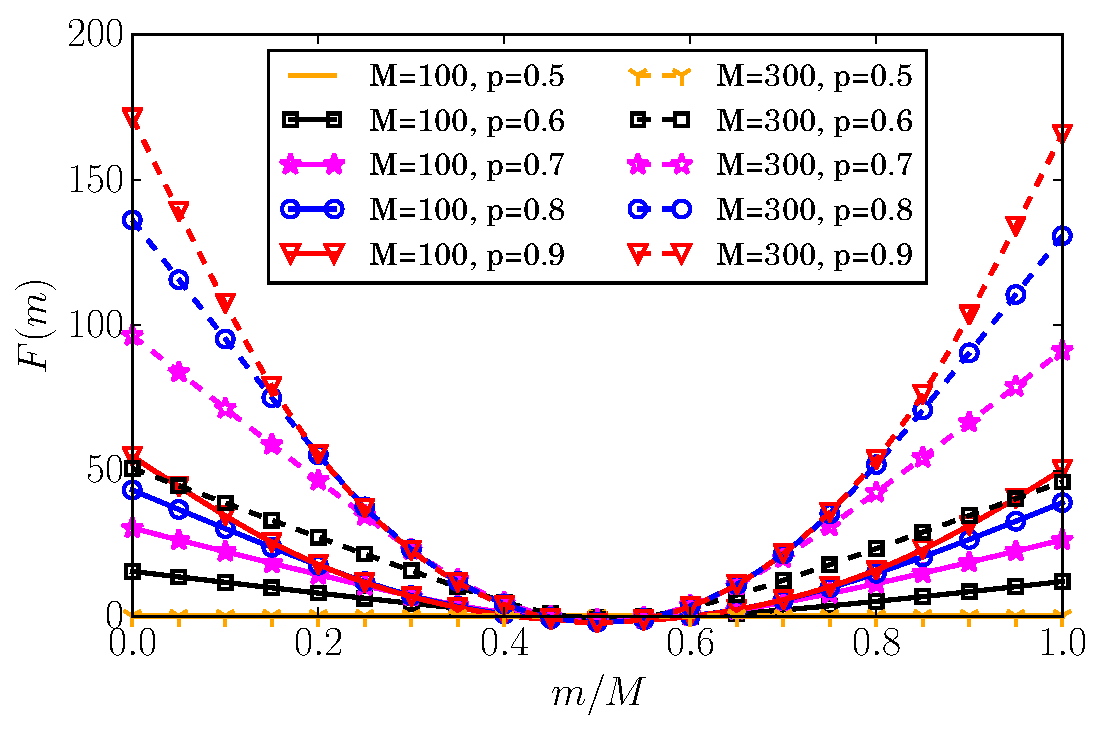
\includegraphics[width=\textwidth]{image/F1}
        \caption{\label{FC1} Curves of $F(m)$}
    \end{subfigure}%
    ~
    \begin{subfigure}[t]{0.24\textwidth}
        \centering
        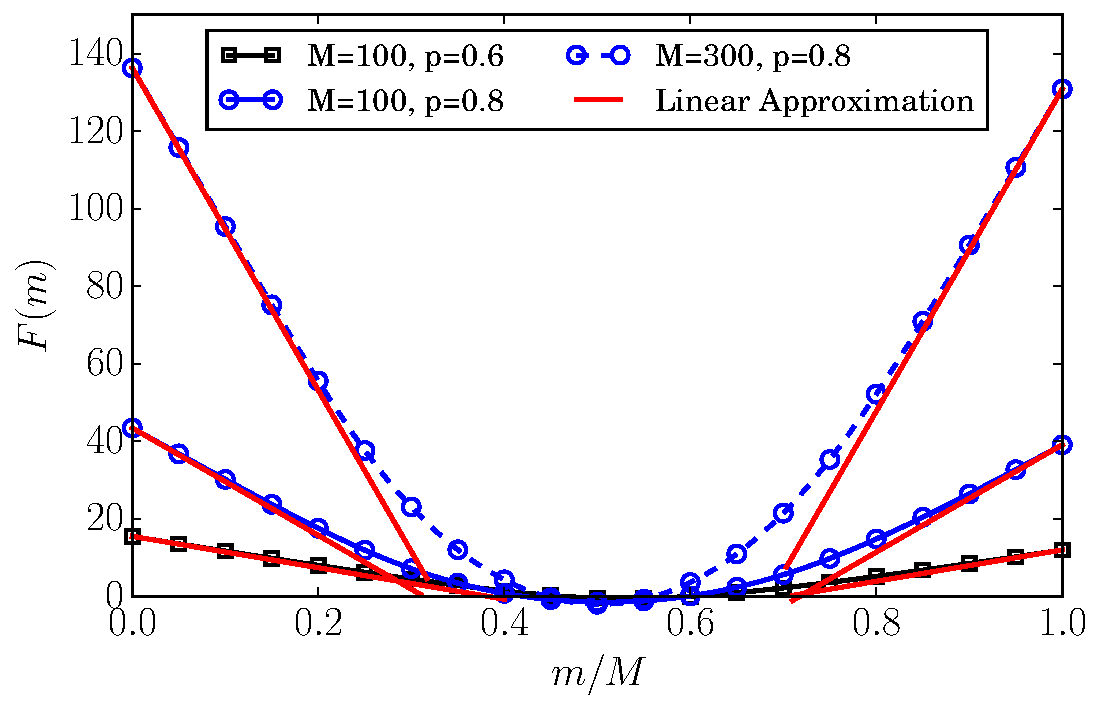
\includegraphics[width=\textwidth]{image/F2}
        \caption{\label{FC2}  Linear Approximation}
    \end{subfigure}
    \caption{\label{FC}Empirical study on $F(m)$}
\end{figure}
\end{proof}
\end{theorem}

Next, we compute $F(0;p)$ as follows:
\begin{equation*}
\begin{split}
&\frac{e^{F(0;p)}}{2^{M+1}}=\sum_{x=0}^{M}C_{M}^{x}p^{x}(1-p)^{y}B(x+2,y+1)\\
&=\frac{(1-p)^{M}}{(M+1)(M+2)}\sum_{x=0}^{M}(x+1)\lambda^{x}\\
&=\frac{(1-p)^{M}}{(M+1)(M+2)}\cdot \frac{\mathrm{d}}{\mathrm{d}\lambda}\sum_{x=0}^{M}\lambda^{x+1}\\
&=\frac{(1-p)^{M+2}-(M+2)(1-p)p^{M+1}+(M+1)p^{M+2}}{(M+1)(M+2)(1-2p)^2}
\end{split}
\end{equation*}
where $\lambda=p/(1-p)$. When $M$ is very large, we can have the following approximation:
\begin{itemize}
\item When $p>0.5$, 
\begin{equation*}
F(0;p)\approx (M+1)\log(2p)-\log(M)-\log|2p-1|.
\end{equation*}
\item When $p=0.5$, $F(0;p)=0$.
\item When $p<0.5$,
\begin{equation*}
\begin{split}
F(0;p)\approx &(M+1)\log(2-2p)\\
&-2\log(M)+\log(1-p)-2\log|2p-1|.
\end{split}
\end{equation*}
\end{itemize}
Considering the symmetry of $F(m;p)$, we can have
\begin{itemize}
\item When $p>0.5$, 
\begin{equation*}
\begin{split}
F(M;p)\approx &(M+1)\log(2p)\\
&-2\log(M)+\log(p)-2\log|2p-1|.
\end{split}
\end{equation*}
\item When $p=0.5$, $F(0;p)=0$.
\item When $p<0.5$,
\begin{equation*}
F(0;p)\approx (M+1)\log(2-2p)-\log(M)-\log|2p-1|.
\end{equation*}
\end{itemize}
Then, we can have
\begin{equation}
   F(0,p)-F(M,p)\approx
    \left\{
    \begin{array}{cl}
    \log(M) & p>0.5\\
    0 & p=0.5\\
    -\log(M) & p<0.5
    \end{array}\right..
\end{equation}

\begin{figure*}[t]
    \centering
    \begin{subfigure}[t]{0.32\textwidth}
        \centering
        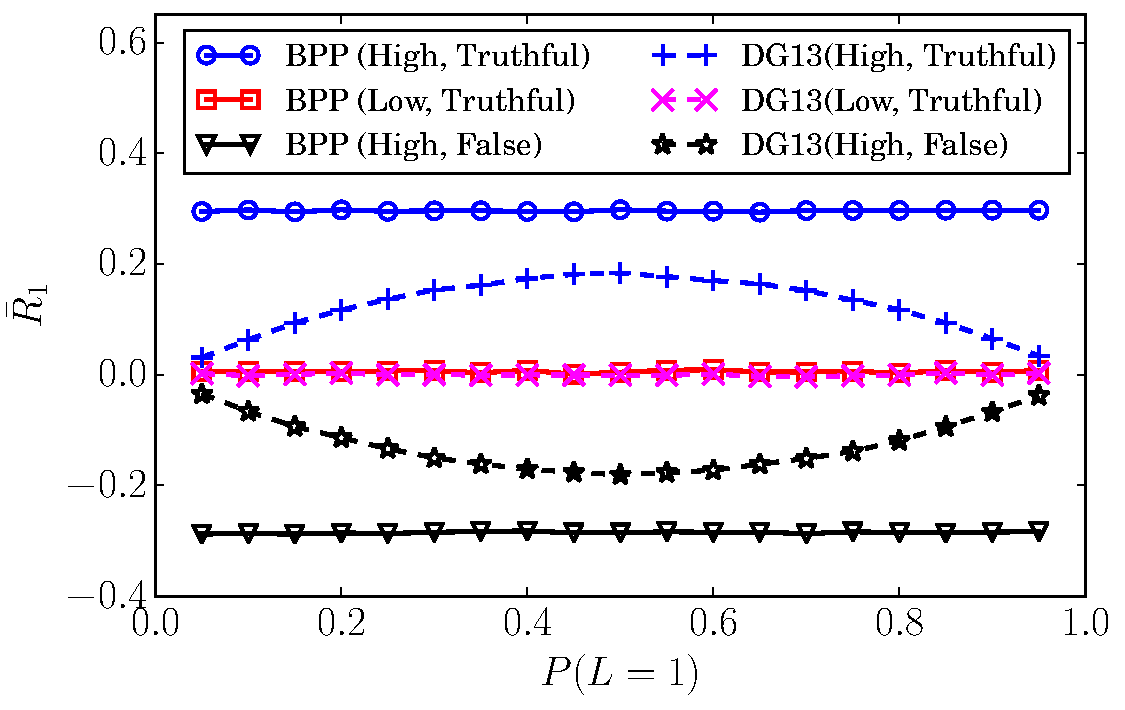
\includegraphics[width=\textwidth]{image/BPP1}
        \caption{\label{BPP1}Changing the true label distribution}
    \end{subfigure}%
    ~
    \begin{subfigure}[t]{0.32\textwidth}
        \centering
        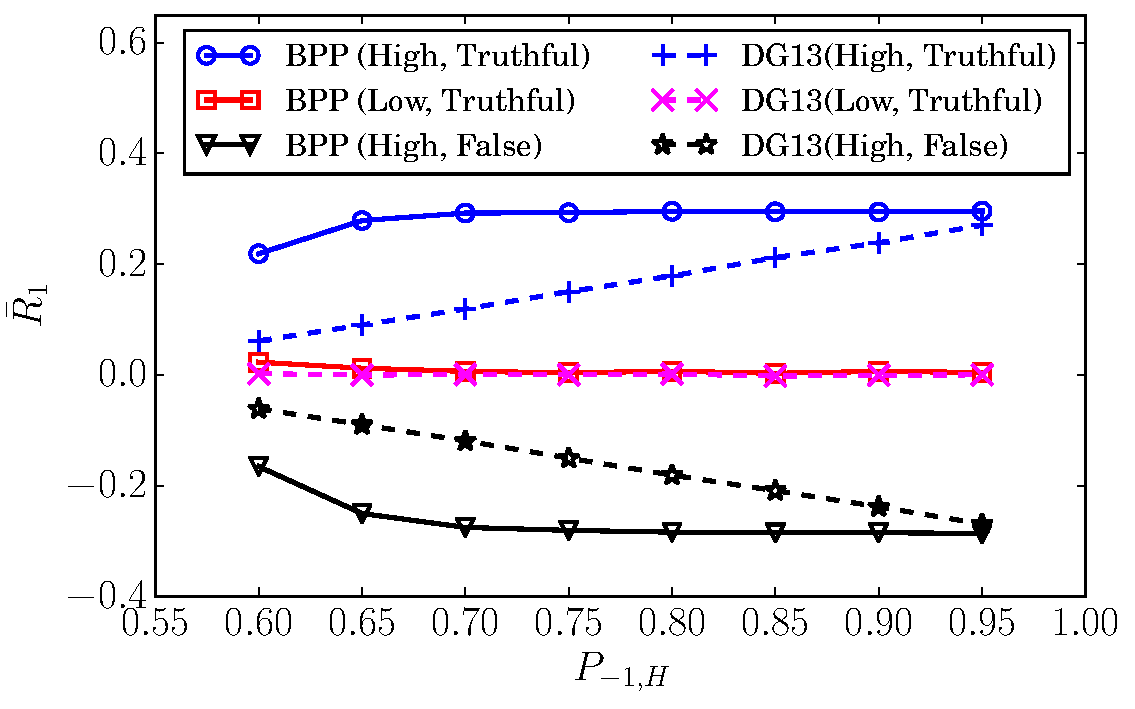
\includegraphics[width=\textwidth]{image/BPP2}
        \caption{\label{BPP2}Changing the opponent workers}
    \end{subfigure}
        ~
    \begin{subfigure}[t]{0.32\textwidth}
        \centering
        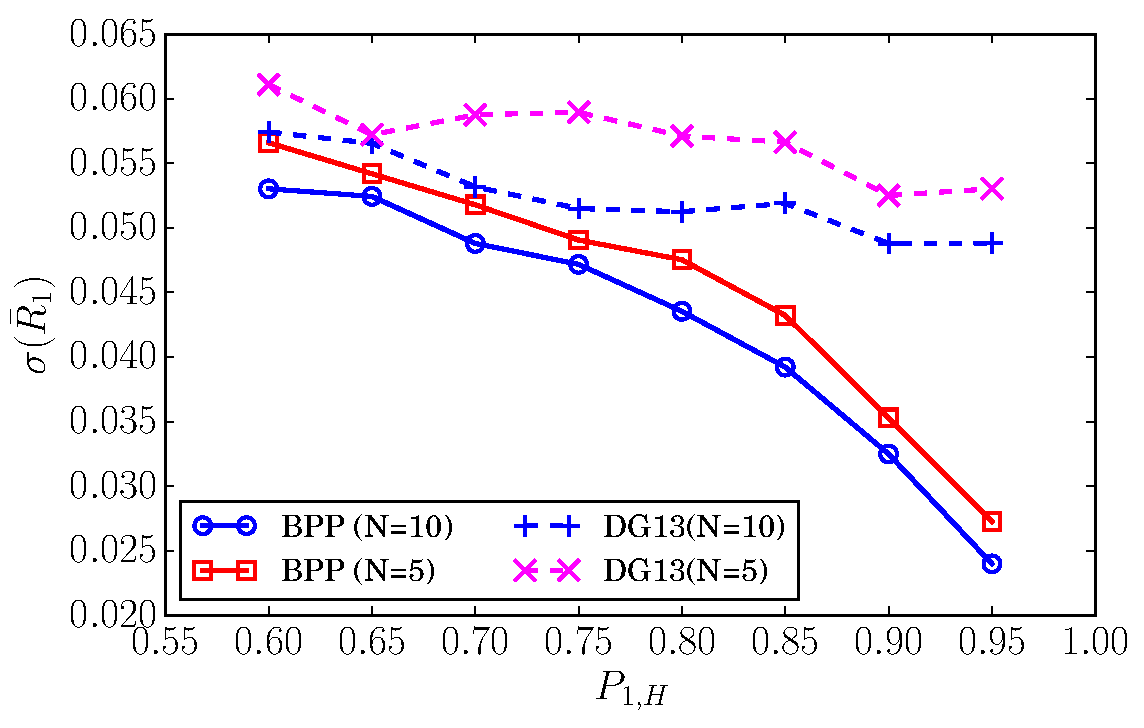
\includegraphics[width=\textwidth]{image/BPP3}
        \caption{\label{BPP3}Changing the targeted worker}
    \end{subfigure}
    \caption{\label{BPP}Empirical analysis on the incentive received by worker $1$}
\end{figure*}

Furthermore, we compute $F(1,p)$ as follows:
\begin{equation*}
\begin{split}
\frac{e^{F(1;p)}}{2^{M+1}}=&\sum_{x=0}^{M-1}C_{M-1}^{x}p^{x}(1-p)^{y+1}B(x+3,y+1)+\\
&\quad \sum_{x=0}^{M-1}C_{M-1}^{x}p^{x+1}(1-p)^{y}B(x+2,y+2)\\
=&\frac{p(1-p)^{M-1}}{M(M+1)}\sum_{x=0}^{M-1}(x+1)\lambda^x + \\
&\quad \frac{(1-2p)(1-p)^{M-1}}{M(M+1)(M+2)}\sum_{x=0}^{M-1}(x+1)(x+2)\lambda^{x}
\end{split}
\end{equation*}
\begin{equation*}
\sum_{x=0}^{M-1}(x+1)\lambda^x =\frac{\mathrm{d}}{\mathrm{d}\lambda}\sum_{x=0}^{M-1}\lambda^{x+1} =\frac{\mathrm{d}}{\mathrm{d}\lambda}\left( \frac{\lambda-\lambda^{M+1}}{1-\lambda}\right)
\end{equation*}
\begin{equation*}
\sum_{x=0}^{M-1}(x+1)(x+2)\lambda^{x} =\frac{\mathrm{d}^2}{\mathrm{d}^2\lambda}\left( \frac{\lambda^2-\lambda^{M+2}}{1-\lambda}\right)
\end{equation*}
When $M$ is very large, we approximate $F(1;p)$ as:
{\color{red}
\begin{itemize}
\item When $p>0.5$, 
\begin{equation*}
F(1;p)\approx M\log(2p)+\log(2-2p+\frac{2}{M})-\log(M)-\log|2p-1|.
\end{equation*}
\item When $p=0.5$, $F(1;p)=0$.
\item When $p<0.5$,
\begin{equation*}
\begin{split}
F(0;p)\approx &(M+1)\log(2-2p)+\log(p+\frac{1}{M})\\
&-2\log(M)+\log(1-p)-2\log|2p-1|.
\end{split}
\end{equation*}
\end{itemize}
}
Thus, the slope of our left-end linear function in Figure~\ref{FC2} can be computed as
\begin{equation}
   k_0\approx
    \left\{
    \begin{array}{cl}
    \log(\lambda) & p>0.5\\
    0 & p=0.5\\
    -\log(\lambda) & p<0.5
    \end{array}\right..
\end{equation}
Using the symmetry of $F(m;p)$, we can prove that the right-end linear function satisfies $k_1=k_0$.


If we define $\rho=m/M$, then we can have
\begin{itemize}
\item When $\rho\leq 0.5$,
\begin{equation}
\sum_{i=1}^{N}F(m;p_i)\approx C-KM\rho
\end{equation}
\item When $\rho>0.5$,
\begin{equation}
\sum_{i=1}^{N}F(m;p_i)\approx C+\delta-KM(1-\rho)
\end{equation}
\end{itemize}
where $$\delta=[n(p_i<0.5)-n(p_i>0.5)]\log(M).$$ Besides, $C=\sum_{i=1}^{N}F(0,p_i)$ and it satisfies
\begin{equation}
\lim_{M\rightarrow \infty}C=+\infty.
\end{equation}
$K=\sum_{i=1}^{N}k_0(p_i)\geq 0$ and the equality holds only when $p_i=0.5$ holds for all workers.
Then, we can compute the expectation as follows:
\begin{equation*}
\begin{split}
\lim_{M\rightarrow \infty}\mathbb{E}\left[\frac{m}{M}\right]=\lim_{M\rightarrow \infty}\sum_{m=0}^{M}\frac{m}{M}P(m)=\lim_{M\rightarrow \infty}\frac{A_1+A_2}{B_1+B_2}
\end{split}
\end{equation*}
where
\begin{equation*}
\begin{split}
A_1&= \sum_{m=0}^{\lfloor0.5M\rfloor}\frac{m}{M} e^{C-Km}\\
&=\frac{e^{C}}{KM}\frac{\mathrm{d}}{\mathrm{d}u}\left.\sum_{m=0}^{\lfloor0.5M\rfloor}u^{Km+1}\right|_{u=e^{-1}}-\frac{1}{KM}B_1\\
&\approx \frac{1+(K+1)e^{-K}}{(1-e^{-K})^2}\cdot \frac{e^C}{KM}-\frac{1}{KM}B_1\\
A_2&=\sum_{m=\lceil0.5M\rceil}^{M}\frac{m}{M} e^{C+\delta-K(M-m)}\\
&= \sum_{u=0}^{\lfloor0.5M\rfloor}\left(1-\frac{u}{M}\right) e^{C+\delta-Ku}= e^{\delta}(B_1-A_1)\\
B_1&=\sum_{m=0}^{\lfloor0.5M\rfloor}e^{C-Km}=\left[1-e^{-0.5KM}\right]e^{C}/(1-e^{-K})\\
B_2&= \sum_{m=\lceil0.5M\rceil}^{M}e^{C+\delta-K(M-m)}=e^{\delta}B_1
\end{split}
\end{equation*}
Thus, when $n(p_i>0.5)>n(p_i<0.5)$,
\begin{equation}
\label{Zero}
\lim_{M\rightarrow \infty}\mathbb{E}\left[\frac{m}{M}\right]=\lim_{M\rightarrow \infty}\frac{1-e^{\delta}}{1+e^{\delta}}G+\frac{e^{\delta}}{1+e^{\delta}}
\end{equation}
where
$$G=\frac{1+(K+1)e^{-K}}{KM(1-e^{-K})(1-e^{-0.5KM})}-\frac{1}{KM}.$$
Thus, 
\begin{equation}
\label{Proof1}
  \lim_{M\rightarrow \infty} |\mathbb{E}_{\mathcal{L}}\hat{p}_i-p_i|\leq \lim_{M\rightarrow \infty} \frac{\mathbb{E}[m]}{M}=0.
\end{equation}
On the other hand, when $n(p_i>0.5)\leq n(p_i<0.5)$,
\begin{equation}
\begin{split}
&\lim_{M\rightarrow \infty} |\hat{p}_i-p_i|\approx \lim_{M\rightarrow \infty} \frac{\mathbb{E}|w_i-z_i|}{M}\\
&= \lim_{M\rightarrow \infty}\mathbb{E}\rho \left|1-\frac{2z_i}{m}\right|\\
&\geq \lim_{M\rightarrow \infty} \sum_{z_i=0}^{M} \left|1-\frac{2z_i}{M}\right|P(z_i|m=M)P(m=M)\\
&= \lim_{M\rightarrow \infty}\sum_{z_i=0}^{M} \left|1-\frac{2z_i}{M}\right|P(z_i|m=M)\frac{e^{C+\delta}}{B_1+B_2}
\end{split}
\end{equation}
where
$$ \lim_{M\rightarrow \infty}\frac{e^{C+\delta}}{B_1+B_2}=\frac{1-e^{K}}{1+e^{\delta}}>1-e^{K}.$$
Besides, $\left|1-\frac{2z_i}{M}\right|\geq 0$ and the equality only holds when $z_i= 0.5M$.
Meanwhile,
$$P(z_i|m=M)=C_{M}^{z_i}p_i^{w_i}(1-p_i)^{z_i}> 0.$$
Thus, when $n(p_i>0.5)\leq n(p_i<0.5)$,
\begin{equation}
\label{Proof2}
\lim_{M\rightarrow \infty} |\mathbb{E}_{\mathcal{L}}\hat{p}_i-p_i|>0.
\end{equation}
Combining Equations~\ref{Proof1} and \ref{Proof2} concludes Theorem~\ref{Conv}.
Then, we prove the incentive compatibility of our Bayesian peer prediction mechanism as follows:
\begin{theorem}
\label{Conv}
When the number of tasks is very large, exerting high efforts ($e_i=1$) and reporting truthfully ($r_i=1$) are a Bayesian Nash equilibrium for all workers.
\begin{proof}
Suppose all workers except worker $i$ exert high efforts and report truthfully. Since we have made the assumption that $p_{j,H}>0.5$ for all $j\in[N]$\footnote{This assumption requires that if workers work exert high efforts, they should be better than random guess. This is a very weak assumption. If it is violated, then the tasks may not suitable for non-expert crowdsourcing workers.}, then $n(p_j>0.5)\geq N-1>n(p_j<0.5)$.
In this case, $\mathbb{E}R(i)\approx M\cdot \left[a\cdot (p_i-0.5) +b\right]$.
Considering Theorem~\ref{Incre}, $\mathbb{E}R(i)$ only reaches the maximum when $e_i=1$ and $r_i=1$.
Thus, worker $i$ will lose her utility if she does not exert high efforts or report falsely. Thus, $(e_i=1,r_i=1)$ is a Bayesian Nash equilibrium for all workers.
\end{proof}
\end{theorem}

\subsection{Empirical Evaluation}
(Empirically Compares with existing ones on stability and fairness. Here, I give an example for the disadvantage of the peer prediction mechanism proposed by~\cite{dasgupta2013crowdsourced}. Suppose all workers always report the fully correct answers by exerting high efforts and report truthfully. Then, if the real true labels are all $1$, then the payment for workers are $0$. If the real true labels are uniformly distributed, the payment are $0.5$. Even though the incentive compatibility is ensured by $\geq$, you see, it has some unreasonable parts which, in principle, can be overcome by our mechanism.)

\section{Reinforcement Bayesian Peer Prediction}
Suppose the true label is $1$.
\begin{equation}
x= \log\frac{P(L=1)}{P(L=2)}=g+\sum_{i=1}^{N}f(x_i,y_i,w_i,z_i)
\end{equation}
\noindent where $g=g_1-g_2$, and 
\begin{equation*}
g_1=\log(s_1+t_2+1)\;,\;g_2=\log(s_2+t_1+1).
\end{equation*}
Omitting the subscript in $f$, we can have $f=f_1-f_2$ with probability $p$ and $f=f_2-f_1$ with probability $1-p$. Here,
\begin{equation*}
f_1=\log(x+z+2)\;,\;f_2=\log(w+y+1).
\end{equation*}
Thus, we can have
\begin{equation}
\mathbb{E}g = \mathbb{E}g_1-\mathbb{E}g_2 \;,\;
\mathbb{E}f = (2p-1)(\mathbb{E}f_1-\mathbb{E}f_2).
\end{equation}
From the previous proof, we know that $P(m)$ is very small when $m>>1$. Thus, we mainly focus on the region where $m$ is relatively small. For a given small $m$,
\begin{equation}
\mathbb{E}_{s_1, t_2}g_1\approx \mathbb{E}_{t_2}\log(np+t_2+1)
\end{equation}
\begin{equation}
\log(np+t_2+1) = \log(np+1)+\sum_{i=1}^{\infty}(-1)^{i-1}q^i
\end{equation}
\begin{equation}
q = \frac{t_2}{np+1}\Rightarrow 0\leq q^{i} \leq c^{i}\cdot \left(\frac{m}{M}\right)^i\leq c^{i}\frac{m}{M}
\end{equation}
Then,
\begin{equation}
\mathbb{E}g_1 \approx \mathbb{E}_{m}\log(1+Mp-mp)
\end{equation}
\begin{equation}
\log(1+Mp-mp)\approx\log(1+Mp)+\sum_{i=1}^{\infty}(-1)^{i}\left(\frac{m}{M}\right)^i
\end{equation}
Using the similar way of approximation for the computation of $\mathbb{E}g_2$, $\mathbb{E}f_1$ and $\mathbb{E}f_2$, we can have
\begin{equation}
\begin{split}
\mathbb{E}g_1\approx \log(Mp)\;,\;\mathbb{E}g_2\approx \log(M(1-p))\\
\mathbb{E}f_1\approx \log(Mp)\;,\;\mathbb{E}f_2\approx \log(M(1-p))
\end{split}
\end{equation}
Thus, if all workers exert high efforts and report truthfully,
\begin{equation}
    \mathbb{E}x \approx \log\lambda_0 + {\sum}_{i=1}^{N}\log\lambda_{i,H}
\end{equation}
If the true label is $2$, then
\begin{equation}
    \mathbb{E}x \approx \log\lambda_0 - {\sum}_{i=1}^{N}\log\lambda_{i,H}
\end{equation}
Thereby,
\begin{equation}
    \mathbb{E}|x|\approx (2p_0-1)\log\lambda_0+ {\sum}_{i=1}^{N}\log\lambda_{i,H}
\end{equation}
When, for example, worker $1$ deviate from the desired equilibrium strategy, the non-equilibrium state correspond to
\begin{equation}
    \mathbb{E}|x'|\approx (2p_0-1)\log\lambda_0+ \log\lambda_{1}+{\sum}_{i=2}^{N}\log\lambda_{i,H}
\end{equation}
The minimal value of $\mathbb{E}|x'|$ is reached when worker $1$ exert high efforts and report falsely, namely $\log\lambda_{i}=-\log\lambda_{i,H}$.
Thus, the maximal reward increment brought by worker $1$'s strategy switch is
\begin{equation}
    V_1 = F(\mathbb{E}x)-F(\mathbb{E}x') \approx 2\log\lambda_{1,H}\cdot \left.\frac{\mathrm{d}F}{\mathrm{d}x}\right|_{x=x_H}
\end{equation}
Since $p_0$ is difficult to estimate, we define the upper bound of the value increment as
\begin{equation}
    V = 2\max_{i}\log\lambda_{i,H} \cdot  \max_{x\in [x_H, \infty)}\frac{\mathrm{d}F}{\mathrm{d}x} 
\end{equation}
where $x_H= \log\lambda_0 + {\sum}_{i=1}^{N}\log\lambda_{i,H}$.
Considering the discounted reward calculation in reinforcement learning, we can know the maximum value difference can be created by the manipulation of any worker is $(1-\rho)^{-1}V$. Meanwhile, if the reinforcement part increases the scaling factor by $\delta$ to obtain the reward increment, we need to pay more than $\sum_{i=1}^{N}M\delta (p_{i,H}-0.5)$. Thus, if we want to prevent the reinforcement learning module from the adversarial manipulation, the minimal gap $\delta$ between to two available scaling factors should satisfy
\begin{equation}
    \sum_{i=1}^{N}M\delta (p_{i,H}-0.5) > V.
\end{equation}

\section{Study the F function}
\begin{lemma}
If $x\sim \mathrm{Bin}(n,p)$, $\mathbb{E}t^x= \left(1-p+tp\right)^{n}$ holds for any $t>0$, where $\mathrm{Bin}(\cdot)$ is the binomial distribution.
\begin{proof}
\begin{equation*}
t^x = e^{x\log t}=m_x(\log t)= \left(1-p+pe^{\log t}\right)^{n}
\end{equation*}
where $m_x(\cdot)$ denotes the moment generating function.
\end{proof}
\end{lemma}

\begin{equation}
B(x+z+2, y+w+1) = \int_{0}^{+\infty} \frac{t^{x+z+1}}{(1+t)^{M+3}}\mathrm{d}t
\end{equation}
Given $n$ and $m$, 
\begin{equation}
\begin{split}
Y=&C_{n}^{x}C_{m}^{w}p_i^{x+w}(1-p)^{y+z}B(x+z+2,y+w+1)\\
&= \int_{0}^{+\infty} \frac{\mathbb{E}_{x,z}t^{x+z+1}}{(1+t)^{M+3}}\mathrm{d}t\\
&=\int_{0}^{+\infty} \frac{(1-p+tp)^n\cdot (p+(1-p)t)^m\cdot t}{(1+t)^{M+3}}\mathrm{d}t\\
&=\int_{1}^{+\infty} \frac{(1-2p+pu)^n\cdot (2p-1+(1-p)u)^m\cdot (u-1)}{u^{M+3}}\mathrm{d}u\\
&=\int_{-1}^{0}[(2p-1)v+p]^{n}[(1-2p)v+1-p]^{m}(1+v)\mathrm{d}v\\
&=\int_{0}^{1}[(2p-1)y+1-p]^{n}[(1-2p)y+p]^{m}y\mathrm{d}y\\
&=\frac{1}{2p-1}\int_{1-p}^{p}x^n(1-x)^m\frac{x-1+p}{2p-1}\mathrm{d}x
\end{split}
\end{equation}
where $x\sim \mathrm{Bin}(n,p)$ and $z\sim \mathrm{Bin}(m,1-p)$. Then,
\begin{itemize}
\item When $n\geq m$ and $p> 0.5$,
\begin{equation}
\begin{split}
Y &\leq  \frac{1}{(2p-1) 2^{2m}}\int_{1-p}^{p}x^{n-m}\mathrm{d}x\\
&= \frac{1}{(2p-1) 2^{2m}}\frac{p^{n-m+1}-(1-p)^{n-m+1}}{n-m+1}\\
&= \frac{p^{n-m+1}}{(2p-1) 2^{2m}}\frac{1-\frac{1}{\lambda^{n-m+1}}}{n-m+1}
\end{split}
\end{equation}
\begin{equation}
\begin{split}
&F=\log(2^{M+1}Y) \\&\leq  (n-m+1)\log(2p)-\log(2p-1)-\log(n-m+1)\\
&=F(0;p)-2m\log(2p)-\log\frac{M-2m+1}{M+1}\\
&\leq F(0;p)-\left[\log(2p)-\frac{\log(M+1)}{M}\right]\cdot 2m\\
&\approx F(0;p)-2m\log(2p)\;\;\text{(when M is very large)}
\end{split}
\end{equation}
\item When $n<m$ and $p>0.5$,
\begin{equation}
\begin{split}
Y &\leq  \frac{1}{(2p-1) 2^{2n}}\int_{1-p}^{p}(1-x)^{m-n}\frac{x-1+p}{2p-1}\mathrm{d}x\\
&= \frac{1}{(2p-1)^2 2^{2n}}\int_{1-p}^{p}y^{m-n}(p-y)\mathrm{d}y
\end{split}
\end{equation}
\begin{equation}
\begin{split}
&\int_{1-p}^{p}y^{m-n}(p-y)\mathrm{d}y\\
&=p\frac{p^{m-n+1}-(1-p)^{m-n+1}}{m-n+1}-\frac{p^{m-n+2}-(1-p)^{m-n+2}}{m-n+2}\\
&\leq \frac{p^{m-n+2}}{(m-n+1)(m-n+2)}
\end{split}
\end{equation}
\begin{equation}
\begin{split}
&F=\log(2^{M+1}Y) \\&\leq  (n-m+1)\log(2p)+\log(p)-2\log(2p-1)-2\log(n-m+1)\\
&=F(M;p)-\left[\log(2p)-2\frac{\log(M+1)}{M}\right]\cdot 2n\\
&\approx F(M;p)-2(M-m)\log(2p)\;\;\text{(when M is very large)}
\end{split}
\end{equation}
\end{itemize}
Besides,
\begin{equation}
\begin{split}
Y(m,n, 1-p)&=\frac{1}{(1-2p)^2}\int_{p}^{1-p}x^m(1-x)^n(x-p)\mathrm{d}x\\
&=\frac{1}{(1-2p)^2}\int_{p}^{1-p}y^{n}(1-y)^{m}(1-y-p)\mathrm{d}y\\
&=\frac{1}{(1-2p)^2}\int_{1-p}^{p}y^{n}(1-y)^{m}(y-1+p)\mathrm{d}y\\
&=Y(n,m,p)
\end{split}
\end{equation}
Thereby, we mainly focus on the cases where $p>0.5$.
On the other hand, there exists $c\in [1-p, p]$ ensuring
\begin{equation}
\begin{split}
&\int_{1-p}^{p}x^{n}(1-x)^{m}(x-1+p)\mathrm{d}y\\
&=\int_{1-p}^{p}\frac{x}{1-x}x^{n-1}(1-x)^{m+1}(x-1+p)\mathrm{d}y\\
&=\frac{c}{1-c}\int_{1-p}^{p}x^{n-1}(1-x)^{m+1}(x-1+p)\mathrm{d}y
\end{split}
\end{equation}
Thus, 
\begin{equation}
\frac{1-p}{p}Y(n,m,p)\leq  Y(n-1,m+1, p) \leq \frac{p}{1-p}Y(n,m,p)
\end{equation}
Therefore,
\begin{itemize}
\item When $n\geq m$ and $p>0.5$
\begin{equation}
F(m;p)\geq F(0;p)-m\log(\lambda)
\end{equation}
\item When $n<m$ and $p>0.5$
\begin{equation}
F(m;p)\geq F(M;p)-(M-m)\log(\lambda)
\end{equation}
where $\lambda = \max \left\{\frac{p}{1-p},\frac{1-p}{p}\right\}$.
\end{itemize}
\textbf{\color{red} Combining the above analysis together, we can have:}
\begin{equation}
\underline{f}(m;p)\leq F(m,p) \leq \overline{f}(m;p)
\end{equation}
where
\begin{equation*}
\underline{f}(m;p)= \left\{
    \begin{array}{cl}
    F(0;p)-\underline{k} m & m\leq 0.5M\\
    F(M;p)-\underline{k}(M-m) & m>0.5M
    \end{array}\right.
\end{equation*}
\begin{equation*}
\overline{f}(m;p)= \left\{
    \begin{array}{cl}
    F(0;p)-\overline{k} m & m\leq 0.5M\\
    F(M;p)-\overline{k}(M-m) & m>0.5M
    \end{array}\right.
\end{equation*}
Here, $\underline{k}=\log(\lambda)$ and $\overline{k}=2\max\{\log(2p),\log(2-2p)\}$.
Therefore,
\begin{itemize}
\item When $2m\leq M$,
\begin{equation}
C-\underline{K}m\leq \sum_{i=1}^{N}F(m;p_i)\leq C-\overline{K}m
\end{equation}
\item When $2m>M$,
\begin{equation}
C+\delta-\underline{K}(M-m)\leq \sum_{i=1}^{N}F(m;p_i)\leq C+\delta-\overline{K}(M-m)
\end{equation}
\end{itemize}
where $$\delta=[n(p_i<0.5)-n(p_i>0.5)]\log(M)$$
$$\underline{K}=\sum_{i=1}^{N}\underline{k_i}\;,\;\overline{K}=\sum_{i=1}^{N}\overline{k_i}$$
Thus,
\begin{equation}
\begin{split}
\mathbb{E}\left[\frac{m}{M}\right]=\sum_{m=0}^{M}\frac{m}{M}P(m)\leq\frac{\overline{A}_1+\overline{A}_2}{\underline{B}_1+\underline{B}_2}
\end{split}
\end{equation}
where
\begin{equation*}
\begin{split}
\overline{A}_1&= \sum_{m=0}^{\lfloor0.5M\rfloor}\frac{m}{M} e^{C-\overline{K}m}\\
\overline{A}_2&=\sum_{m=\lceil0.5M\rceil}^{M}\frac{m}{M} e^{C+\delta-\overline{K}(M-m)}\\
\underline{B}_1&=\sum_{m=0}^{\lfloor0.5M\rfloor}e^{C-\underline{K}m}\\
\underline{B}_2&= \sum_{m=\lceil0.5M\rceil}^{M}e^{C+\delta-\underline{K}(M-m)}
\end{split}
\end{equation*}
Using the same method as Equation~\ref{Zero} to solve the sum, we can get the same conclusion as before.
\bibliographystyle{named}
\bibliography{ref}



\end{document}

